\chapter{LE2ML: un \textit{workbench} modulaire pour l'apprentissage machine}
\label{chap:6}

\section{Introduction}

\section{État de l'art}

\subsection{WEKA}

\begin{figure}[H]
	\centering
	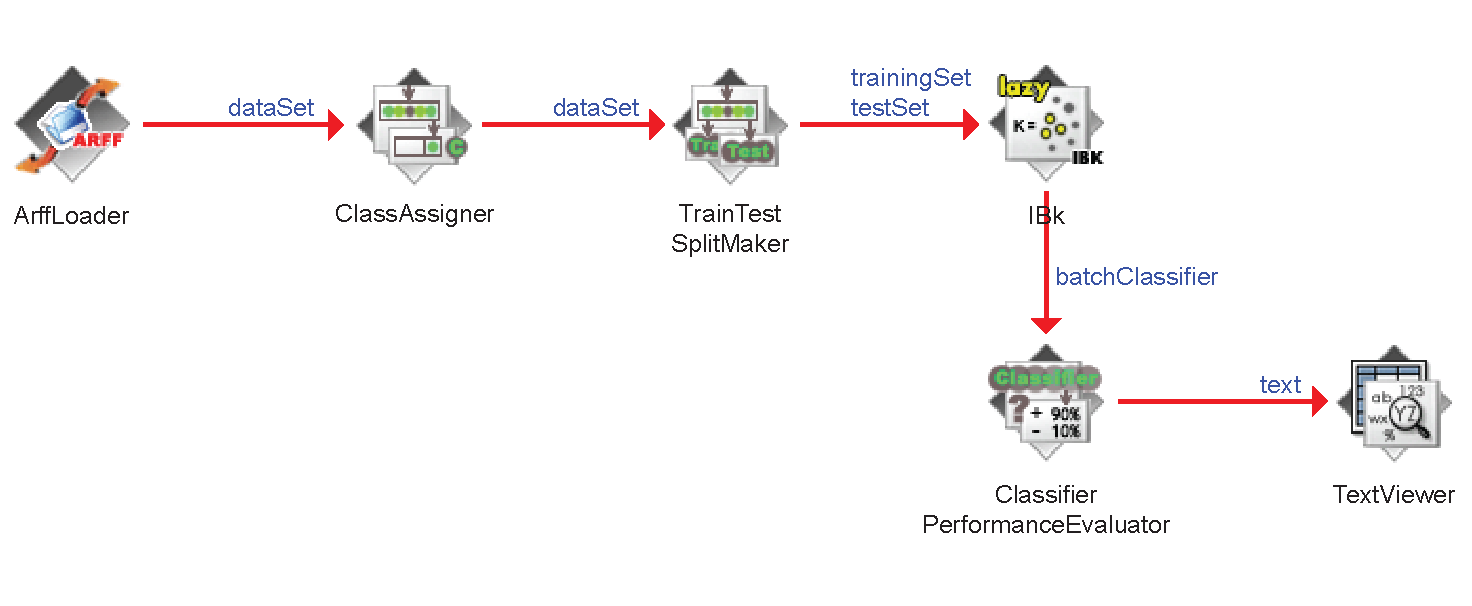
\includegraphics[width=.8\linewidth]{chapter6/weka.pdf}
        \caption{caption}
	\label{fig:weka}
\end{figure}

\subsection{RapidMiner}

\begin{figure}[H]
	\centering
	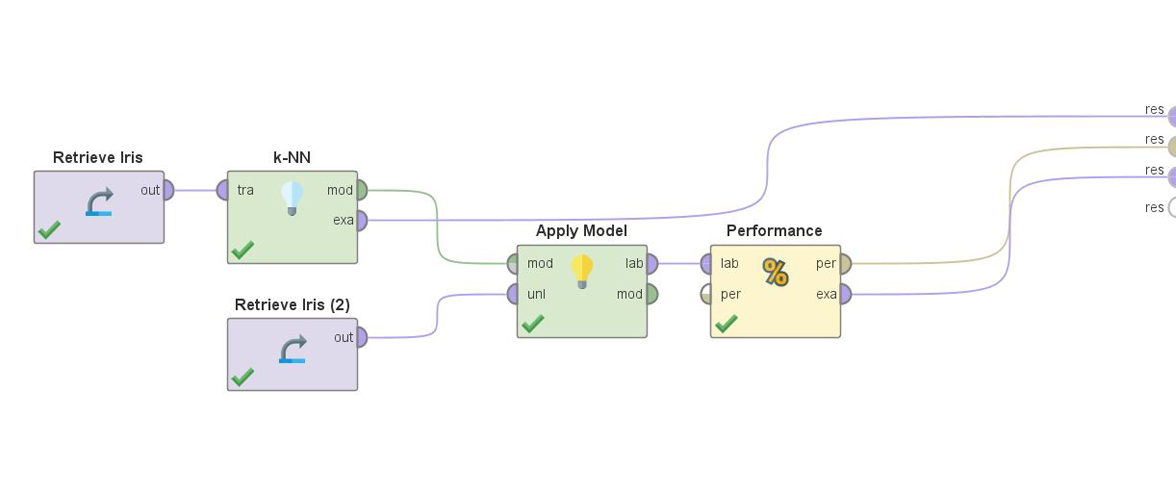
\includegraphics[width=.8\linewidth]{chapter6/rapid_miner.jpg}
        \caption{caption}
	\label{fig:rapid_miner}
\end{figure}

\subsection{Orange}

\begin{figure}[H]
	\centering
	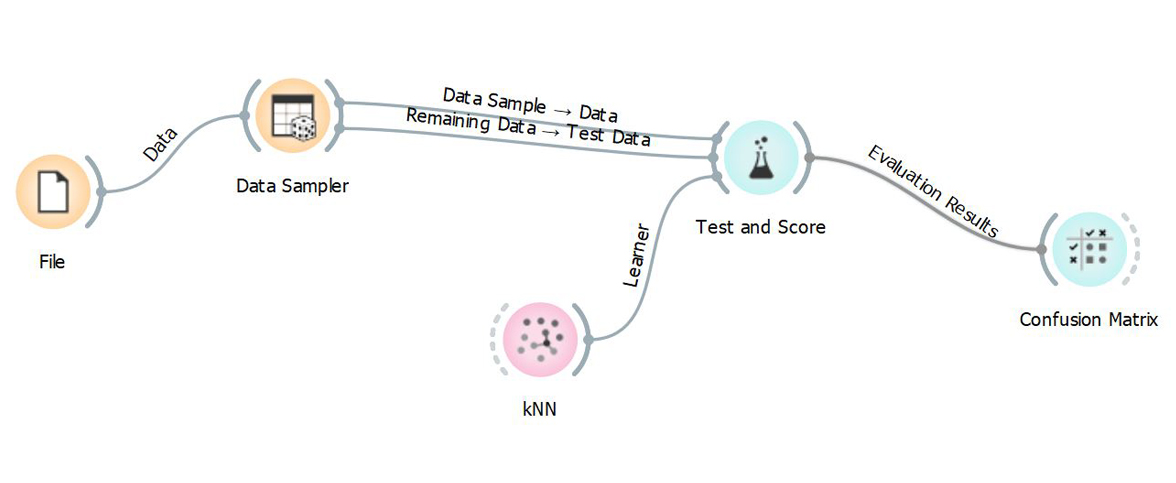
\includegraphics[width=.8\linewidth]{chapter6/orange.jpg}
        \caption{caption}
	\label{fig:orange}
\end{figure}

\subsection{Conclusion}

\section{Solution proposée}

\begin{figure}[H]
	\centering
	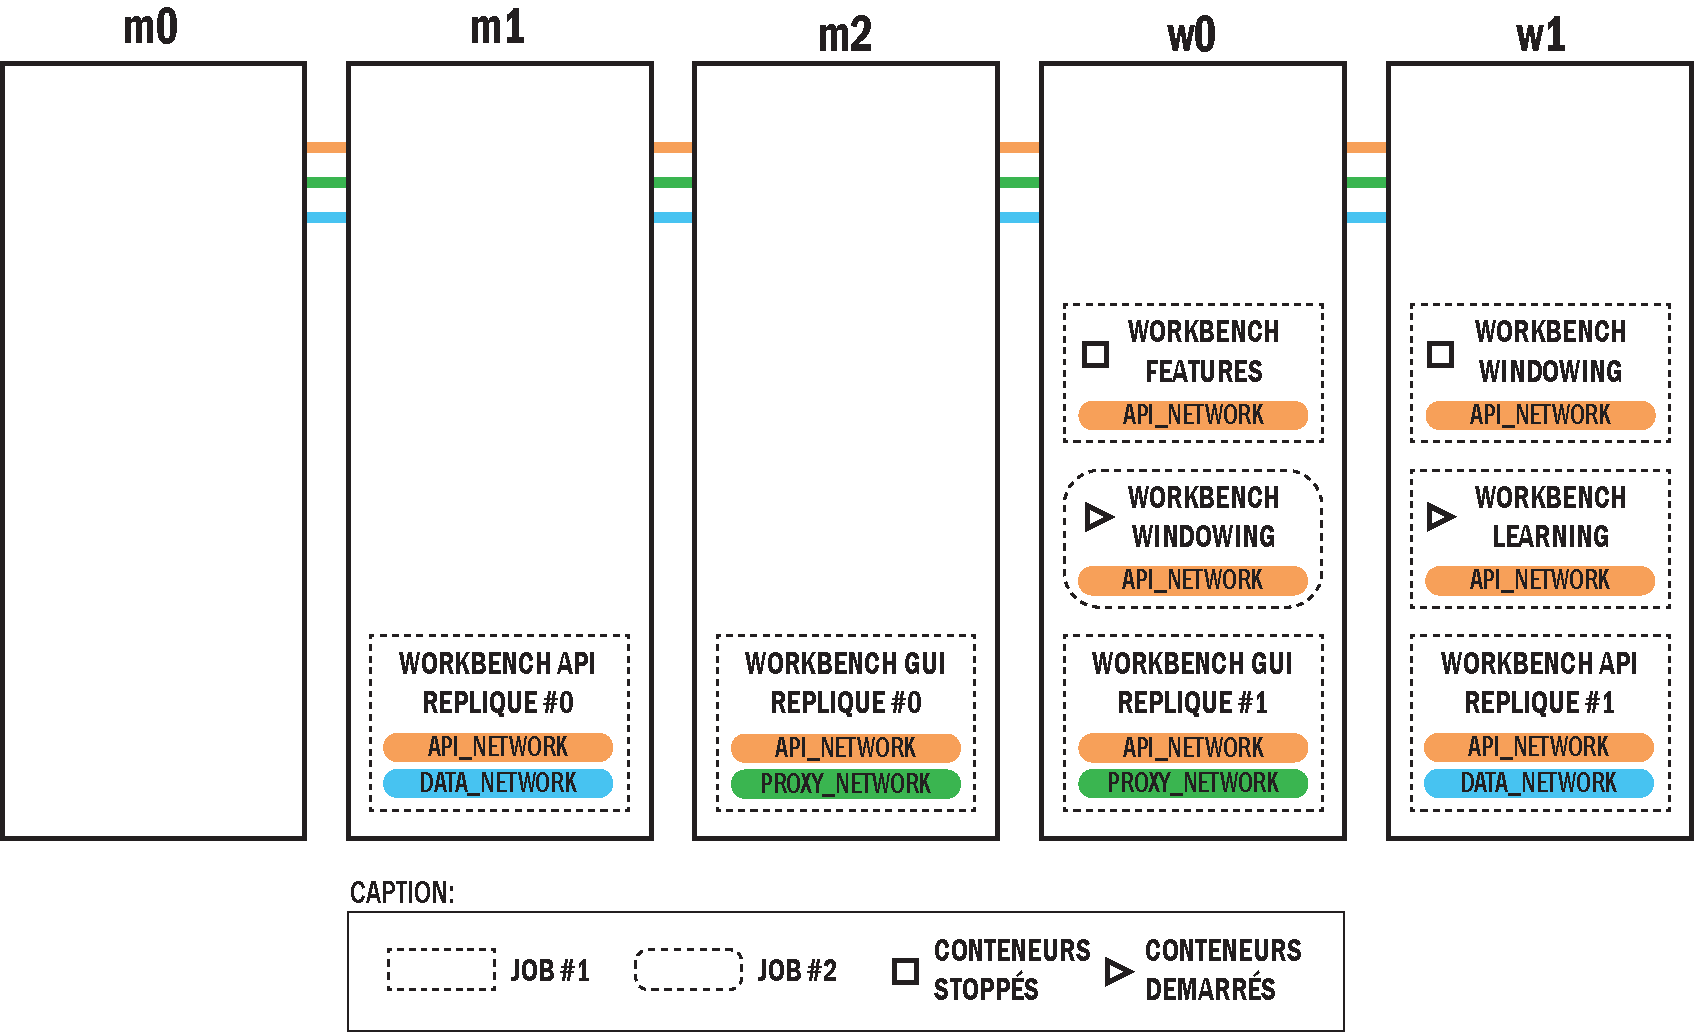
\includegraphics[width=.8\linewidth]{chapter6/containers_workbench.pdf}
        \caption{caption}
	\label{fig:containers_workbench}
\end{figure}

\subsection{API REST}

\begin{figure}[H]
	\centering
	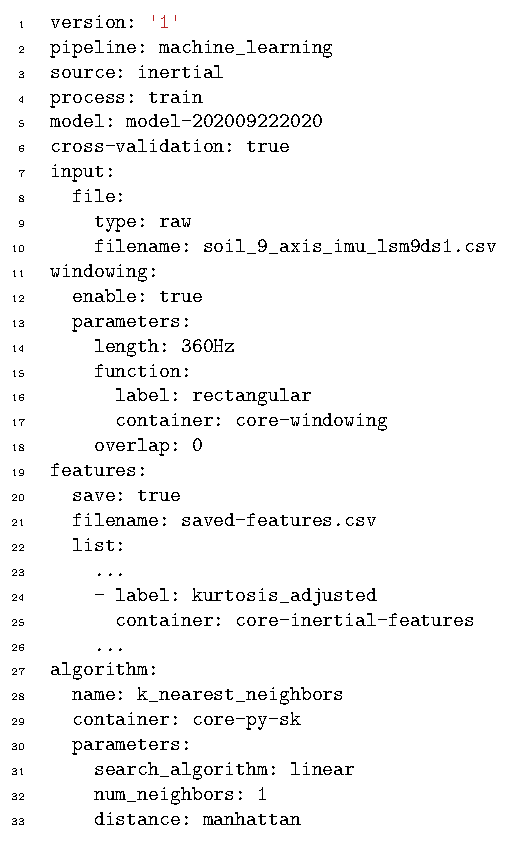
\includegraphics[width=.5\linewidth,keepaspectratio]{chapter6/pipeline_conf.pdf}
        \caption{caption}
	\label{fig:pipeline_conf}
\end{figure}

\subsection{Application Web}

\begin{figure}[H]
	\centering
	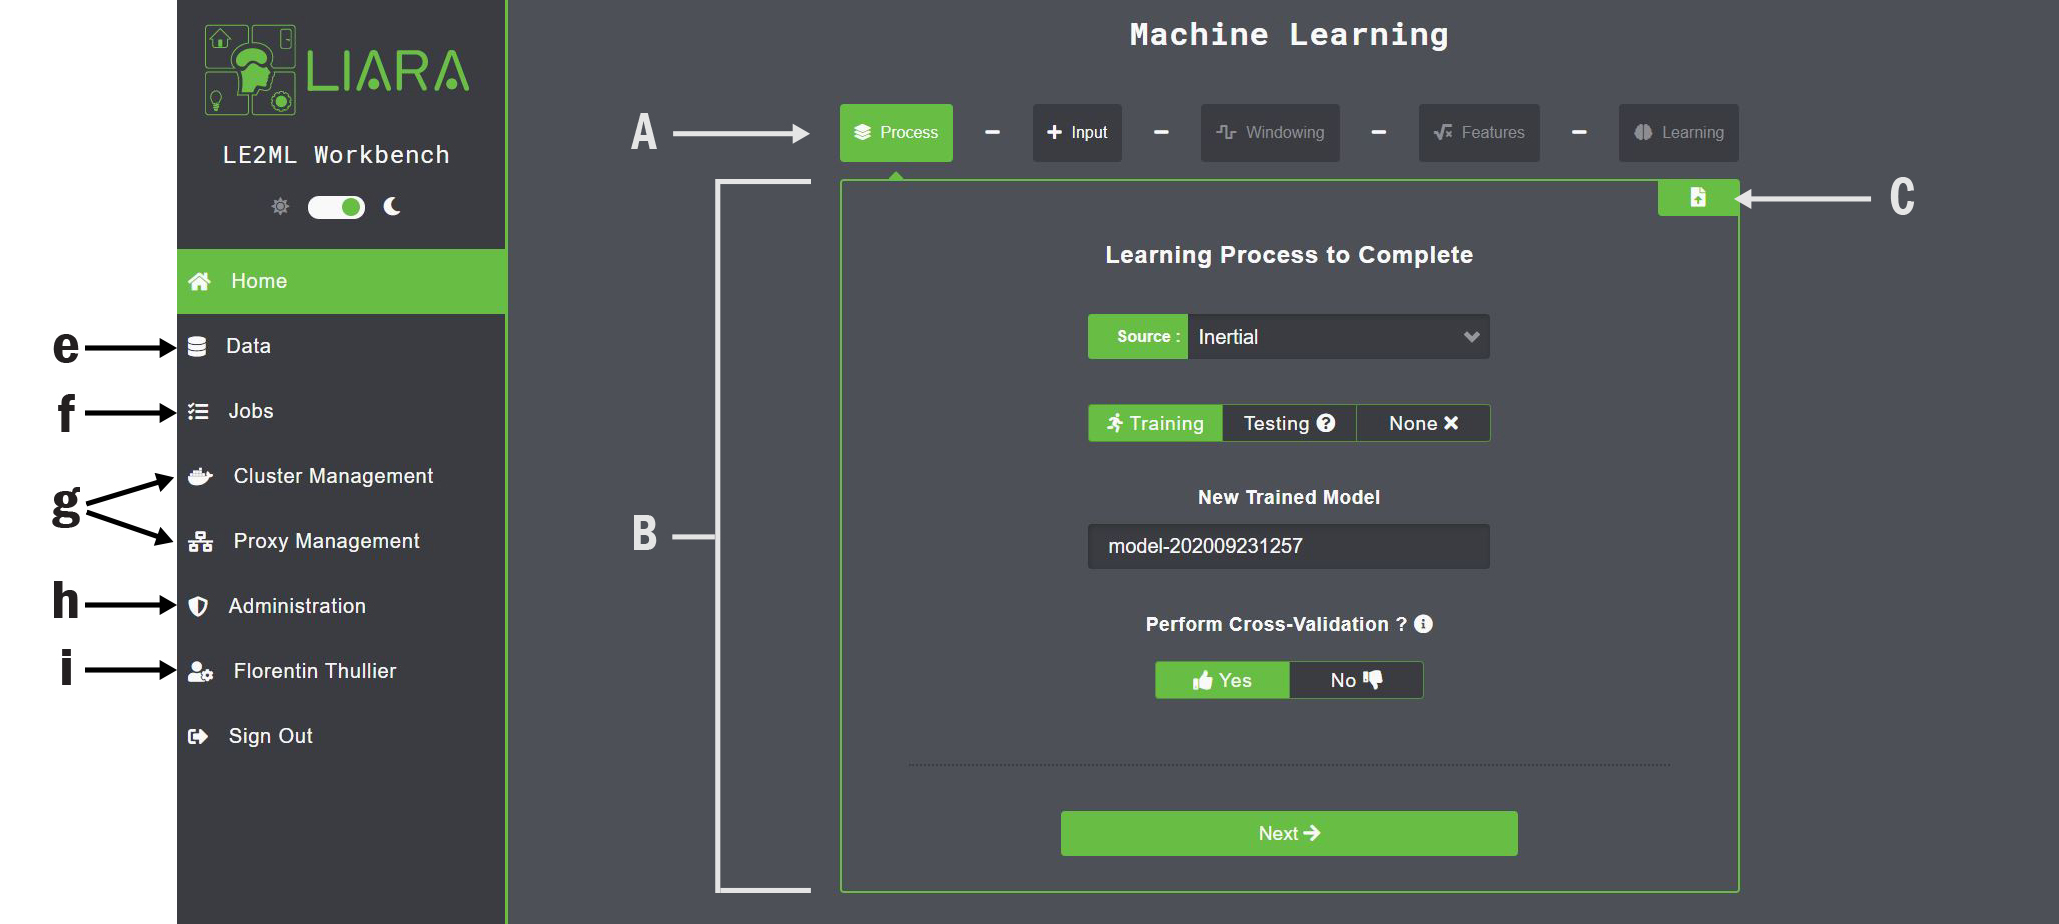
\includegraphics[angle=90,origin=c,height=\textwidth,keepaspectratio]{chapter6/le2ml_gui.jpg}
        \caption{caption}
	\label{fig:le2ml_gui}
\end{figure}

\subsection{Modules proposés}

\subsubsection{Fenêtrage}

\subsubsection{Extraction de caractéristiques}

\subsubsection{Apprentissage machine}

\section{Expérimentations \& Résultats}

\begin{table}[H]
    \centering
    \caption{caption.}
    \label{tab:previous_results}
    \begin{tabular}{@{}rccc@{}}
      \toprule
      \multicolumn{1}{l}{}  & Justesse  &  $F\mbox{-} mesure$  & $k$    \\ \midrule
      \texttt{k-NN}         & 0.93      & 0.93                & 0.89    \\
      Random Forest         & 0.92      & 0.92                & 0.88    \\ \bottomrule
    \end{tabular}
\end{table}

\begin{table}[H]
    \centering
    \caption{caption.}
    \label{tab:l2ml_results}
    \begin{tabular}{@{}rccc@{}}
      \toprule
      \multicolumn{1}{l}{}  & Justesse  &  $F\mbox{-} mesure$  & $k$    \\ \midrule
      \texttt{k-NN}         & 0.91      & 0.91                & 0.86    \\
      Random Forest         & 0.92      & 0.92                & 0.88    \\ \bottomrule
    \end{tabular}
\end{table}

\section{Conclusion}